
\chapter{The \plasTeX\ Document\label{sec:document}}

The \plasTeX\ document is very similar to an XML DOM structure.  In fact,
you can use XML DOM methods to create and populate nodes, delete or move
nodes, etc.  The biggest difference between the \plasTeX\ document and
an XML document is that in XML the attributes of an element are simply 
string values, whereas attributes in a \plasTeX\ document are generally 
document fragments that contain the arguments of a macro.  Attributes can
be canfigured to hold other Python objects like lists, dictionaries, and
strings as well (see the section \ref{sec:macros} for more information).

While XML document objects have a very strict syntax, \LaTeX\ documents
are a little more free-form.  Because of this, the \plasTeX\ framework
does a lot of normalizing of the \LaTeX\ document to make it conform to
a set of rules.  This set of rules means that you will always get a 
consistent output document which is necessary for easy manipulation and
programability.

The overall document structure should not be surprising.  There is a 
document element at the top level which corresponds to the XML Document
node.  The child nodes of the Document node begin with the preamble to 
the \LaTeX\ document.  This includes things like the \macro{documentclass},
\macro{newcommand}s, \macro{title}, \macro{author}, counter settings, etc.
For the most part, these nodes can be ignored.  While they are a useful
part of the document, they are generally only used by internal processes
in \plasTeX.  What is important is the last node in the document which
corresponds to \LaTeX's \environment{document} environment.

The \environment{document} environment has a very simple structure.  
It consists solely of paragraphs (actually \macro{par}s in \TeX's terms) 
and sections\footnote{``sections'' in
this document is used loosely to mean any type of section: part, chapter, 
section, etc.}.  In fact, all sections have this same format including
parts, chapters, sections, subsections, subsubsections, paragraphs, and
subparagraphs.  \plasTeX\ can tell which pieces of a document correspond
to a sectioning element by looking at the \member{level} attribute of the
Python class that corresponds to the given macro.  The section levels in
\plasTeX\ are the same as those used by \LaTeX: -1 for part, 0 for chapter,
1 for section, etc.  You can create your own sectioning commands simply
by subclassing an existing macro class, or by setting the \member{level}
attribute to a value that corresponds to the level of section you want
to mimic.  All level values less than 100 are reserved for sectioning so
you aren't limited to \LaTeX's sectioning depth.  Figure \ref{fig:docstructure} 
below shows an example of the overall document structure.

\begin{figure}[ht]
\begin{center}
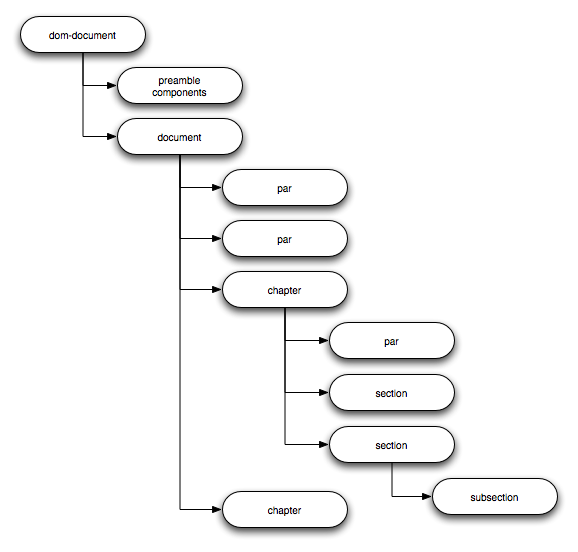
\includegraphics[width=4in]{docstructure}
\end{center}
\caption{The overall \plasTeX\ document structure\label{fig:docstructure}}
\end{figure}

This document is constructed during the parsing process by calling the 
\method{digest} method on each node.  The \method{digest} method is passed
an iterator of document nodes that correspond to the nodes in the document
that follow the current node.  It is the 
responsibility of the current node to only absorb the nodes that belong
to it during the digest process.  Luckily, the default \method{digest}
method will work in nearly all cases.  See section \ref{sec:macros} for more
information on the digestion process.

Part of this digestion process is grouping nodes into paragraphs.  This
is done using the \method{paragraphs} method available in all \class{Macro}
based classes.  This method uses the same technique as \TeX\ to group
paragraphs of content.  Section \ref{sec:paragraphs} has more information
about the details of paragraph grouping.

In addition to the \member{level} attribute of sections, there is also a
mixin class that assists in generating the table of contents and navigation
elements during rendering.  If you create your own sectioning commands,
you should include \class{plasTeX.Base.LaTeX.Sectioning.SectionUtils} as
a base class as well.  All of the standard \LaTeX\ section commands already
inherit from this class, so if you subclass one of those, you'll get
the helper methods for free.  For more information on these helper methods
see section \ref{sec:sections}.

The structure of the rest of the document is also fairly simple and 
well-defined.  \LaTeX\ commands are each converted into a document node
with it's arguments getting placed into the \member{attributes} dictionary.
\LaTeX\ environments also create a single node in the document, where
the child nodes of the environment include everything between the 
\macro{begin} and \macro{end} commands.  By default, the child nodes of
an environment are simply inserted in the order that they appear in the 
document.  However, there are some environments that require further
processing due to their more complex structures.  These structures include
arrays and tabular environments, as well as itemized lists.  For more
information on these structures see sections \ref{sec:arrays} and
\ref{sec:lists}, respectively.  Figures \ref{fig:docfragcode} and 
\ref{fig:docfrag} shows a common \LaTeX\ document fragment and the 
resulting \plasTeX\ document node structure.

\begin{figure}[ht]
\begin{verbatim}
\begin{center}
Every \textbf{good} boy does \textit{fine}.
\end{center}
\end{verbatim}
\caption{Sample \LaTeX\ document fragment code\label{fig:docfragcode}}
\end{figure}

\begin{figure}[ht]
\begin{center}
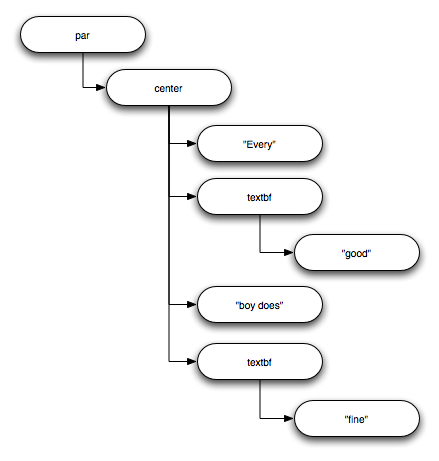
\includegraphics[width=3in]{docfrag}
\end{center}
\caption{Resulting \plasTeX\ document node structure\label{fig:docfrag}}
\end{figure}

You may have noticed that in the document structure in Figure \ref{fig:docfrag}
the text corresponding to the argument for \macro{textbf} and \macro{textit} 
is actually a child node and not an attribute.  This is actually a 
convenience feature in \plasTeX.  For macros like this where there is only
one argument and that argument corresponds to the content of the macro,
it is common to put that content into the child nodes.  This is done in
the \member{args} attribute of the macro class by setting the argument's
name to ``self''.  This magical value will link the attribute called 
``self'' to the child nodes array.  For more information on the \member{args}
attribute and how it populates the \member{attributes} dictionary see
section \ref{sec:macros}.

In the \plasTeX\ framework, the input \LaTeX\ document is parsed and 
digested until the document is finished.  At this point, you should have
an output document that conforms to the rules described above.  The 
document should have a regular enough structure that working with it
programatically using DOM methods or Python practices should be fairly
straight-forward.  The following sections give more detail on document
structure elements that require extra processing beyond the standard
parse-digest process.


\section{Sections\label{sec:sections}}

``Sections'' in \plasTeX\ refer to any macro that creates a section-like
construct in a document including the \environment{document} environment,
\macro{part}, \macro{chapter}, \macro{section}, \macro{subsection}, 
\macro{subsubsection}, \macro{paragraph}, and \macro{subparagraph}.
While these are the sectioning macros defined by \LaTeX, you are not limited
to using just those commands to create sections in your own documents.
There are two elements that must exist for a Python macro class to act
like a section: 1) the \member{level} attribute must be set to a value
less than 100, and 2) the class should inherit from 
\class{plasTeX.Base.LaTeX.Sectioning.SectionUtils}.

The \member{level} attribute refers to the section level in the document.
The values for this attribute are the same values that \LaTeX\ uses
for its section levels, namely:
\begin{description}
\item[-1 {\it or} \member{Node.PART_LEVEL}] corresponds to \macro{part}
\item[0 {\it or} \member{Node.CHAPTER_LEVEL}] corresponds to \macro{chapter}
\item[1 {\it or} \member{Node.SECTION_LEVEL}] corresponds to \macro{section}
\item[2 {\it or} \member{Node.SUBSECTION_LEVEL}] corresponds to \macro{subsection}
\item[3 {\it or} \member{Node.SUBSUBSECTION_LEVEL}] corresponds to \macro{subsubsection}
\item[4 {\it or} \member{Node.PARAGRAPH_LEVEL}] corresponds to \macro{paragraph}
\item[5 {\it or} \member{Node.SUBPARAGRAPH_LEVEL}] corresponds to \macro{subparagraph}
\end{description}

\plasTeX\ adds the following section related levels:
\begin{description}
\item[-\code{sys.maxint} {\it or} \member{Node.DOCUMENT_LEVEL}] 
    corresponds to the \environment{document} environment and 
    is always the top-level section
\item[6 {\it or} \member{Node.SUBSUBPARAGRAPH_LEVEL}]
    this level was added to correspond to the sixth level of headings
    defined in HTML
\item[100 {\it or} \member{Node.ENDSECTIONS_LEVEL}]
    flag that indicates the last possible section nesting level.  This is 
    mainly used for internal purposes.
\end{description}

\plasTeX\ uses the \member{level} attribute to build the appropriate 
document structure.  If all you need is a proper document structure,
the \member{level} attribute is the only thing that needs to be set on
a macro.  However, there are many convenience properties in the 
\class{plasTeX.Base.LaTeX.Sectioning.SectionUtils} class that are used
in the rendering process.  
If you plan on rendering your document, your
section classes should inherit from this class.  Below is a list
of the additional properties and their purpose.
\begin{tableii}{l|p{4in}}{member}{Name}{Purpose}
\lineii{allSections}{contains a sequential list of all of the sections 
    within and including the current section}
\lineii{documentSections}{contains a sequential list of all of the
    sections within the entire document}
\lineii{links}{contains a dictionary contain various amounts of 
    navigation information corresponding mostly to the link types 
    described at \url{http://fantasai.tripod.com/qref/Appendix/LinkTypes/ltdef.html}.
    This includes things like breadcrumb trails, previous and next links,
    links to the overall table of contents, etc.  See section \ref{sec:links}
    for more information.}
\lineii{siblings}{contains a list of all of the sibling sections}
\lineii{subsections}{contains a list of all of the sections within 
    the current section}
\lineii{tableofcontents}{contains an object that corresponds to the
    table of contents for the section.  The table of contents is 
    configurable as well.  For more information on how to configure
    the table of contents see section \ref{sec:tableofcontents}}
\end{tableii}
\note{When first accessed, each of these properties actually navigates the
      document and builds the returned object.  Since these operations
      can be rather costly, the values are cached.  Therefore, if you
      modify the document after accessing one of these properties you
      will not see the change reflected.}


\subsection{Navigation and Links\label{sec:links}}

The \class{plasTeX.Base.LaTeX.Sectioning.SectionUtils} class has a
property named \member{links} that contains a dictionary of many useful
objects that assist in creating navigation bars and breadcrumb trails
in the rendered output.  This dictionary was modeled after the links
described at \url{http://fantasai.tripod.com/qref/Appendix/LinkTypes/ltdef.html}.
Some of the objects in this dictionary are created automatically, others
are created with the help of the \member{linkType} attribute on the 
document nodes, and yet others can be added manually from a configuration
file or command-line options.  The automatically generated values are 
listed in the following table.
\begin{tableii}{l|p{4in}}{var}{Name}{Purpose}
\lineii{begin}{the first section of the document}
\lineii{breadcrumbs}{a list containing the entire parentage of the 
    current section (including the current section)}
\lineii{chapter}{the current chapter node}
\lineii{child}{a list of the subsections}
\lineii{contents}{the section that contains the top-level table of contents}
\lineii{document}{the document level node}
\lineii{end}{the last section of the document}
\lineii{first}{the first section of the document}
\lineii{home}{the first section of the document}
\lineii{home}{the first section of the document}
\lineii{last}{the last section of the document}
\lineii{navigator}{the section that contains the top-level table of contents}
\lineii{next}{the next section in the document}
\lineii{origin}{the section that contains the top-level table of contents}
\lineii{parent}{the parent node}
\lineii{part}{the current part node}
\lineii{prev}{the previous section in the document}
\lineii{previous}{the previous section in the document}
\lineii{section}{the current section}
\lineii{sibling}{a list of the section siblings}
\lineii{subsection}{the current subsection}
\lineii{start}{the first section of the document}
\lineii{toc}{the section that contains the top-level table of contents}
\lineii{top}{the first section of the document}
\lineii{up}{the parent section}
\end{tableii}
\note{The keys in every case are simply strings.}
\note{Each of the elements in the table above is either a section node or a list
of section nodes.  Of course, once you have a reference to a node you can
acces the attributes and methods of that object for further introspection.}
An example of accessing these objects from a section instance is shown below.
\begin{verbatim}
previousnode = sectionnode.links['prev']
nextnode = sectionnode.links['next']
\end{verbatim}

The next method of populating the links table is semi-automatic and uses
the \member{linkType} attribute on the Python macro class.  There are 
certain parts of a document that only occur once such as an index, 
glossary, or bibliography.  You can set the \member{linkType} attribute
on the Python macro class to a string that corresponds to that sections 
role in the document (i.e. `index' for the index, `glossary' for the glossary,
`bibliography' for the bibliography).  When a node with a special link
type is created, it is inserted into the dictionary of links with the 
given name.  This allows you to have links to indexes, glossaries, etc.
appear in the links object only when they are in the current document.
The example below shows the \environment{theindex} environment being
configured to show up under the `index' key in the links dictionary.
\begin{verbatim}
class theindex(Environment, SectionUtils):
    nodeType = 'index'
    level = Environment.SECTION_LEVEL
\end{verbatim}
\note{These links are actually stored under the `links' key of the
      owner document's userdata dictionary (i.e. 
      \code{self.ownerDocument.userdata['links'])}. Other objects can
      be added to this dictionary manually.}

The final way of getting objects into the links dictionary is through 
a configuration file or command-line options.  This method is described
fully in section \ref{sec:config-links}.


\subsection{Table of Contents\label{sec:tableofcontents}}

The table of contents object returned by the \member{tableofcontents}
property of \class{SectionUtils} is not an actual node of the document,
but it is a proxy object that limits the number of levels that you can
traverse.  The number of levels that you are allowed to traverse is
determined by \configkeys{document}{toc-depth} section of the configuration
(see section \ref{sec:config-document}).  Other than the fact that you
can only see a certain number of levels of subsections, the object 
otherwise acts just like any other section node.

In addition to limiting the number of levels of a table of contents,
you can also determine whether or not sections that do not generate new
files while rendering should appear in the table of contents.  By
default, only sections that generate a new file while rendering will
appear in the table of contents object.  If you set the value of
\configkeys{document}{toc-non-files} in the configuration to \code{True},
then all sections will appear in the table of contents.


\section{Paragraphs\label{sec:paragraphs}}

Paragraphs in a \plasTeX\ document are grouped in the same way that they
are grouped in \TeX: essentially anything within a section that isn't a
section itself is put into a paragraph.  This is different than the HTML
model where tables and lists are not grouped into paragraphs.  Because
of this, it is likely that HTML generated that keeps the same paragraph
model will not be 100\% valid.  However, it is highly unlikely that this 
variance from validity will cause any real problems in the browser 
rendering the correct output.

Paragraphs are grouped using the \method{paragraphs} method available on
all Python macro classes.  When this method is invoked on a node, 
all of the child nodes are grouped into paragraphs.  If there are no
paragraph objects in the list of child nodes already, one is created.
This is done to make sure that the document is fully normalized and 
that paragraphs occur everywhere that they can occur.  This is
most noteworthy in constructs like tables and lists where some table cells
or list items have multiple paragraphs and others do not.  If a paragraph
weren't forced into these areas, you could have inconsistently 
paragraph-ed content.

Some areas where paragraphs are allowed, but not necessarily needed might
not want the forced paragraph to be generated, such as within a grouping
of curly braces (\{~\}).  In these cases, you can
use the \code{force=False} keyword argument to \method{paragraphs}.
This still does paragraph grouping, but only if there is a paragraph element
already in the list of child nodes.


\section{Complex Structures\label{sec:complexdoc}}

While much of a \plasTeX\ document mirrors the structure of the source
\LaTeX\ document, some constructs do require a little more work to be
useful in the more rigid structure.  The most noteworthy of these 
constructs are lists, arrays (or tabular environments), and indexes.  
These objects are described in more detail in the following sections.


\subsection{Lists\label{sec:lists}}

Lists are normalized slightly more than the rest of the document.
They are treated almost like sections in that they are only allowed to
contain a minimal set of child node types.  In fact, lists can only
contain one type of child node: list item.  The consequence of this is that
any content before the first item in a list will be thrown out.  In turn, 
list items will only contain paragraph nodes.  The structure of all
list structures will look like the structure in Figure \ref{fig:liststruct}.

\begin{figure}[ht]
\begin{center}
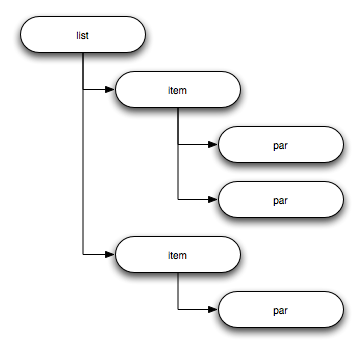
\includegraphics[width=3in]{liststruct}
\end{center}
\caption{Normalized structure of all lists\label{fig:liststruct}}
\end{figure}

This structure allows you to easily traverse a list with code like the
following.
\begin{verbatim}
# Iterate through the items in the list node
for item in listnode:

    # Iterate through the paragraphs in each item
    for par in item:

        # Print the text content of each paragraph
        print par.textContent

    # Print a blank line to separate each item
    print
\end{verbatim}

\subsection{Bibliography}

The bibliography is really just another list structure with a few 
enhancements to allow referencing of the items throughout the document.
Bibliography processing is left to the normal tools.  \plasTeX\
expects a properly \file{.bbl} file for the bibliography.  
The \LaTeX\ bibliography is the format used by default; however, 
the natbib package is also included with \plasTeX\ for more 
complex formatting of bibliographies.


\subsection{Arrays and Tabular Environments\label{sec:arrays}}

Arrays and tabular environments are the most complex structures in a 
\plasTeX\ document.  This because tables can include spanning columns,
spanning rows, and borders specified on the table, rows, and individual 
cells.  In addition, there are alignments associated with each column
and alignments can be specified by any \macro{multicolumn} command.
It is also possible with some packages to create your own column 
declarations.  Add to that the fact that the longtable package allows
you to specify multiple headers, footers, and coptions, and you can see
why tabular environments can be rather tricky to deal with.

As with all parts of the document, \plasTeX\ tries to normalize all tables
to have a consistent structure.  The structure for arrays and tables is 
shown in Figure \ref{fig:tablestruct}.
\begin{figure}[ht]
\begin{center}
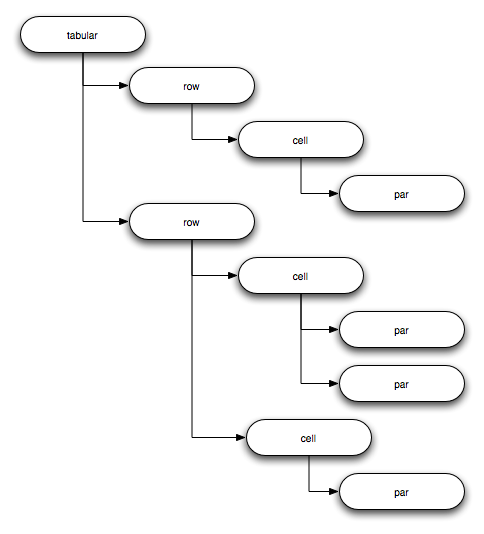
\includegraphics[width=4in]{tablestruct}
\end{center}
\caption{Normalized structure of all tables and arrays\label{fig:tablestruct}}
\end{figure}

Luckily, the array macro class that comes with \plasTeX\ was made to handle
all of the work for you.  In fact, it also handles the work of some extra 
packages such as longtable to make processing them transparent. The details
of the tabular environments are described in the following sections.

With this normalized structure, you can traverse all array and table 
structures with code like the following.
\begin{verbatim}
# Iterate through all rows in the table
for row in tablenode:

    # Iterate through all cells in the row
    for cell in row:

        # Iterate through all paragraphs in the cell
        for par in cell:

            # Print the text content of each cell
            print '   ' + par.textContent 

        # Print a blank line after each cell
        print

    # Print a blank line after each row
    print
\end{verbatim}


\subsubsection{Borders}

Borders in a tabular environment are generally handled by \macro{hline},
\macro{vline}, \macro{cline}, as well as the column specifications on 
the tabular environment and the \macro{multicolumn} command.  
\plasTeX\ merges all of the border specifications and puts them into 
CSS formatted values in the \member{style} attribute of each of the 
table cell nodes.  To get the CSS information formatted such that it
can be used in an inline style, simply access the \member{inline} property
of the style object. 

Here is an example of a \environment{tabular} environment.
\begin{verbatim}
\begin{tabular}{|l|l|}\hline
x & y \\
1 & 2 \\\hline
\end{tabular}
\end{verbatim}

The table node can be traversed as follows.
\begin{verbatim}
# Print the CSS for the borders of each cell
for rownum, row in enumerate(table):
    for cellnum, cell in enumerate(row):
        print '(%s,%s) %s -- %s' % (rownum, cellnum, 
               cell.textContent.strip(), cell.style.inline)
\end{verbatim}

The code above will print the following output (whitespace has been added
to make the output easier to read).
\begin{verbatim}
(0,0) x -- border-top-style:solid; 
           border-left:1px solid black; 
           border-right:1px solid black; 
           border-top-color:black; 
           border-top-width:1px; 
           text-align:left
(0,1) y -- border-top-style:solid; 
           text-align:left; 
           border-top-color:black; 
           border-top-width:1px; 
           border-right:1px solid black
(1,0) 1 -- border-bottom-style:solid; 
           border-bottom-width:1px; 
           border-left:1px solid black; 
           border-right:1px solid black; 
           text-align:left; 
           border-bottom-color:black
(1,1) 2 -- border-bottom-color:black; 
           border-bottom-width:1px; 
           text-align:left; 
           border-bottom-style:solid; 
           border-right:1px solid black
\end{verbatim}


\subsubsection{Alignments}

Alignments can be specified in the column specification of the tabular 
environment as well as in the column specification of \macro{multicolumn}
commands.  Just like the border information, the alignment information
is also stored in CSS formatted values in each cell's \member{style}
attribute.


\subsubsection{Longtables}

Longtables are treated just like regular tables.  Only the first header
and the last footer are supported in the resulting table structure.
To indicate that these are verifiable header or footer cells, the 
\member{isHeader} attribute of the corresponding cells is set to 
\code{True}.  This information can be used by the renderer to more 
accurately represent the table cells.


\subsection{Indexes}

All index building and sorting is done internally in \plasTeX.  It is 
done this way because the information that tools like \program{makeindex}
generate is only useful to \LaTeX\ itself since the refence to the 
place where the index tag was inserted is simply a page number.  Since
\plasTeX\ wants to be able to reference the index tag node, it has 
to do all of the index processing natively.

There are actually two index structures.  The default structure is simply 
the index nodes sorted and grouped into the appropriate hierarchies.
This structure looks like the structure pictured in Figure 
\ref{fig:defaultindex}.
\begin{figure}[ht]
\begin{center}
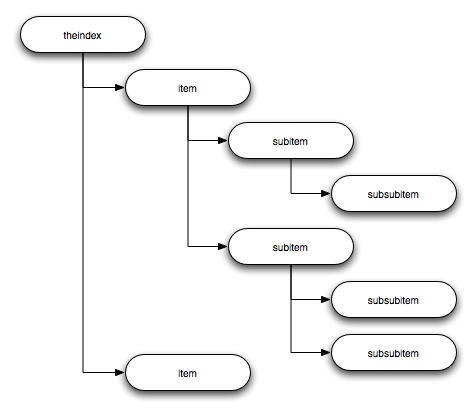
\includegraphics[width=4in]{defaultindex}
\end{center}
\caption{Default index structure\label{fig:defaultindex}}
\end{figure}

Each item, subitem, and subsubitem has an attribute called \member{key}
that contains a document fragment of the key for that index item.
The document nodes that this key corresponds to are held in a list
in the \member{pages} attribute.  These nodes are the actual 
nodes corresponding to the index entry macros from the \LaTeX\ document.
The content of the node is a number corresponding to the index entry
that is formatted according to the formatting rules specified in the
index entry.

While the structure above works well for paged media, it is sometimes 
nice to have the index entries grouped by first letter and possibly
even arranged into multiple columns.  This alternate representation
can be accessed in the \member{groups} property.  The structure 
for this type of index is shown in Figure \ref{fig:groupedindex}.
\begin{figure}[ht]
\begin{center}
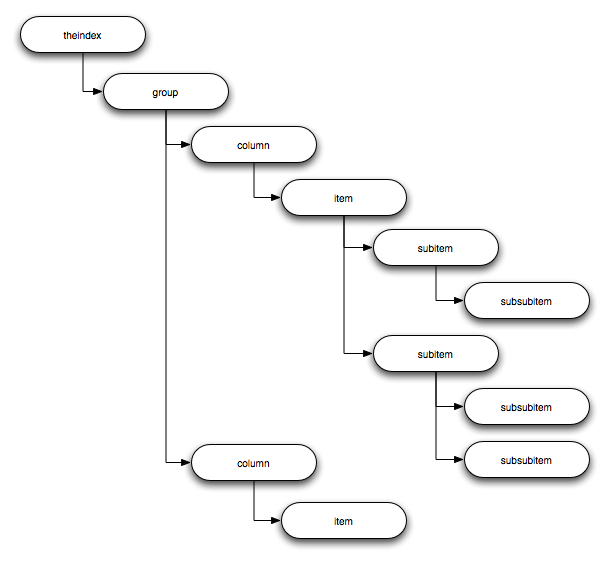
\includegraphics[width=4in]{groupedindex}
\end{center}
\caption{Grouped index structure\label{fig:groupedindex}}
\end{figure}

In this case, the item, subitem, and subsubitem nodes are the same as in
the default scheme.  The group has a \member{title} attribute that contains
the first letter of the entries in that group.  Entries that start with
something other than a letter or an underscore are put into a group
called ``Symbols''.  The columns are approximately equally sized columns
of index entries.  The number of columns is determined by the 
\configkeys{document}{index-columns} configuration item.
